\scanpage{7}
\margin{\figure{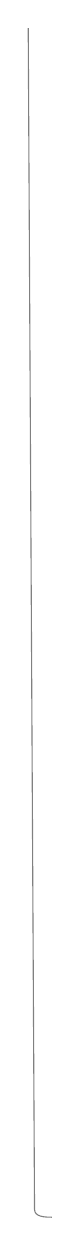
\begin{tikzpicture}\draw[gray] (0,15)--(.08,0) to[out=-90,in=180] (.3,-.1);\end{tikzpicture}}}
\diagram{$(8.5.1)$\quad\begin{tikzcd}[ampersand replacement=\&,column sep=small,row sep=large]
0\arrow[r]\&\operatorname{Ker}v\arrow[r,"\inserted{w}"]\&\deleted{\unsure{\operatorname{Coker}w}}\inserted{\text{\figure{\begin{tikzpicture}[baseline=(n.base)]\node[draw,ellipse] (n) {$({}_p\operatorname{Tors}^n(X))_{\mathrm{ss}}$};\end{tikzpicture}}}}\arrow[r]\&(E(Y)\otimes_W k)_{\mathrm{SS}}\arrow[r,"\inserted{\varphi}"]\&\unsure{E(Y,\underline O_Y)_{\mathrm{SS}}}\arrow[r]\arrow[d,phantom,"\rotatebox{90}{$=$}"]\&\inserted{0}\deleted{\unsure{\operatorname{Ker}w\longrightarrow0}}\\
\&\&\&\&\inserted{\operatorname{Coker}v}\&
\end{tikzcd},}
où on désigne par $v$ l'homomorphisme de restriction
\[
(8.5.2)\qquad v:H^{n-1}(X,\underline O_X)_{\mathrm{SS}}\longrightarrow H^{n-1}(Y,\underline O_Y)_{\mathrm{SS}},
\]
(en particulier $\operatorname{Coker}v$ est la ``cohomologie évanescente cohérente'' $E(Y,\underline O_Y)$), \deleted{et par $w$ l'homomorphisme
\[
(8.5.3)\qquad w:(\operatorname{Tors}^{n-1}(X)\otimes_W k)_{\mathrm{SS}}\xrightarrow{\inserted{u''_2}}(\operatorname{Tors}^{n+1}(X)\otimes_W k)_{\mathrm{SS}}
\]
induit par l'homomorphisme $H^{\unsure{n-1|n+1}}(X)\to H^{n+1}(X)$, \deleted{\unsure{cup}}défini par le cup-produit avec la classe de polarisation \inserted{$d\unsure{\xi|\zeta}$} sur $X$.}
\margin{\figure{\begin{tikzpicture}\node[draw,ellipse] {\unsure{Faux}};\end{tikzpicture}}}
\margin{\unsure{$K_g$} \unsure{fait donc} \illegible{4} \unsure{$V$} \illegible{2} \unsure{nul} sur la}
Enfin, pour utiliser cette suite exacte (8.5.1), on tiendra compte du fait que
\[
(8.5.4)\qquad E(Y)\overset{\mathrm{dfn}}=\operatorname{Coker}(H^{n-1}(X)\to H^{n-1}(Y))\quad\deleted{\unsure{est}}
\]
est un $W$-module libre \uline{sans torsion}; en particulier, si $k$ est un corps fini, le rang de $(E(Y)\otimes_W k)_{\mathrm{SS}}$ est égal au nombre des valeurs propres de Frobenius géométrique relatif à $k$ opérant sur $E^{n-1}(\unsure{Y|X})$ (la cohomologie cristalline évanescente de $Y$; ou ce qui revient au même, la cohomologie $\ell$-adique pour n'importe quel $\ell\ne p$ -- sous réserve de l'algébricité de l'opération $\Lambda$ sur lescohomologies cristallines et $\ell$-adiques) \uline{qui sont des unités $p$-adiques}; les valeurs propres en question, réduites \unsure{modulo} $p$, sont égales aux valeurspropres du frobenius $p$-linéaire (relatif \unsure{au} corps de base fini $k$) opérant sur le terme $E(Y)\otimes_W k$ de (8.5.1), ou si on préfère, en termes de l'interprétation 8.4.2, aux valeurs propres du \inserted{l'inverse du} générateur de frobenius de $G=\operatorname{Gal}(\bar k/k)$ opérant sur le vectoriel de dimension finie sur $\underline F_p$ correspondant.

Notons d'autre part l'égalité suivante déduite de (8.5.1):
\[
\begin{aligned}
(8.5.5)\quad\dim(E(Y)\otimes_W k)_{\mathrm{SS}}={}&\dim E(Y,\underline O_Y)_{\mathrm{SS}}\deleted{\unsure{-\dim\operatorname{Ker}w}}\\
&+(\dim\deleted{\operatorname{Coker}w}\inserted{({}_p\operatorname{Tors}^n(X))_{\mathrm{ss}}}-\dim\operatorname{Ker}v),\quad\unsure{*}
\end{aligned}
\]
où le terme entre parenthèses du deuxième membre est $\geq0$, de sorte \unsure{qu'on}

\mspage{6}
